\documentclass[english,t]{beamer}
% \documentclass[finnish,english,handout]{beamer}

\usepackage[T1]{fontenc}
\usepackage[utf8]{inputenc}
\usepackage{newtxtext} % times
%\usepackage[scaled=.95]{cabin} % sans serif
\usepackage{amsmath}
\usepackage[varqu,varl]{inconsolata} % typewriter
\usepackage[varg]{newtxmath}
\usefonttheme[onlymath]{serif} % beamer font theme
\usepackage{microtype}
\usepackage{url}
\urlstyle{same}
\usepackage{graphicx}
\graphicspath{{./figs/}}
\usepackage{alltt}
\usepackage{subfigure}
\usepackage{enumerate}
\usepackage{listings}

\mode<presentation>
{
  \setbeamercovered{invisible}
  \setbeamertemplate{itemize items}[circle]
  \setbeamercolor{frametitle}{bg=white,fg=navyblue}
  \setbeamertemplate{navigation symbols}{}
  \setbeamertemplate{headline}[default]{}
  \setbeamertemplate{footline}[split]
  % \setbeamertemplate{headline}[text line]{\insertsection}
  % \setbeamertemplate{footline}[frame number]
}

\pdfinfo{            
  /Title      (BDA, Lecture 2) 
  /Author     (Aki Vehtari) % 
  /Keywords   (Bayesian data analysis)
}

% Use tikz
\usepackage{tikz}
\usetikzlibrary{shapes,arrows}

\newenvironment{list1}{
  \begin{list}{$\color{list1}\bullet$}{\itemsep=6pt}}{
  \end{list}}
\newenvironment{list2}{
  \begin{list}{-}{\baselineskip=15pt}}{
  \end{list}}
\newenvironment{list3}{
  \begin{list}{$\cdot$}{\baselineskip=15pt}}{
  \end{list}}

\DeclareMathOperator{\E}{E}
\DeclareMathOperator{\Var}{Var}
\DeclareMathOperator{\var}{var}
\DeclareMathOperator{\Sd}{Sd}
\DeclareMathOperator{\sd}{sd}
\DeclareMathOperator{\Gammad}{Gamma}
\DeclareMathOperator{\Invgamma}{Inv-gamma}
\DeclareMathOperator{\Bin}{Bin}
\DeclareMathOperator{\Negbin}{Neg-bin}
\DeclareMathOperator{\Poisson}{Poisson}
\DeclareMathOperator{\Beta}{Beta}
\DeclareMathOperator{\BetaBinomial}{Beta-Binomial}
\DeclareMathOperator{\logit}{logit}
\DeclareMathOperator{\N}{N}
\DeclareMathOperator{\normal}{normal}
\DeclareMathOperator{\U}{U}
\DeclareMathOperator{\BF}{BF}
\DeclareMathOperator{\Invchi2}{Inv-\chi^2}
% \DeclareMathOperator{\Pr}{Pr}
\def\euro{{\footnotesize \EUR\, }}
\DeclareMathOperator{\rep}{\mathrm{rep}}

\definecolor{navyblue}{rgb}{0,0,0.5}
\definecolor{darkgreen}{rgb}{0,0.3922,0}
\definecolor{matblue}{rgb}{0,0.447,0.741}    
\definecolor{matred}{rgb}{0.85,0.325,0.098}
\definecolor{matyellow}{rgb}{0.929,0.694,0.125}
\definecolor{matpurple}{rgb}{0.494,0.184,0.556}
\definecolor{matgreen}{rgb}{0.466,0.674,0.188}
\definecolor{matcyan}{rgb}{0.301,0.745,0.933}
\definecolor{matdarkred}{rgb}{0.635,0.078,0.184}

\newcommand{\nred}{{\color{matred}\#red}}
\newcommand{\nyellow}{{\color{matyellow}\#yellow}}
\newcommand{\red}{{\color{matred}\#red}}
\newcommand{\yellow}{{\color{matyellow}\#yellow}}

\hypersetup{pdfstartview={FitV}}
\date{}

\title[]{Bayesian data analysis}
\subtitle{}

\author{Aki Vehtari}

\institute[Aalto University]{}

\begin{document} 


\begin{frame}{Outline of Lecture 2}

  \begin{itemize}
  \item Binomial model is the simplest model
    \begin{itemize}
    \item useful to introduce observation model, likelihood,
      posterior, prior, integration, posterior summaries
    \item very commonly used as a building block
    \item examples:
      \begin{itemize}
      \item coin tossing
      \item chips from bag
      \item COVID tests and vaccines
      \item classification / logistic regression
      \end{itemize}
    \end{itemize}
  \end{itemize}
  
\end{frame}

\begin{frame}

  \frametitle{Outline of Chapter 2}

  \begin{itemize}
  \item 2.1 Binomial model (repeated experiment with binary outcome)
  \item 2.2 Posterior as compromise between data and prior information
  \item 2.3 Posterior summaries
  \item 2.4 Informative prior distributions (skip exponential families and sufficient statistics)
  \item 2.5 Gaussian model with known variance
  \item 2.6 Other single parameter models
    \begin{itemize}
    \item the normal distribution with known mean but
      unknown variance is the most important
    \item glance through Poisson and exponential
    \end{itemize}
  \item 2.7 glance through this example, which illustrates benefits of prior information, no need to read all the details (it's quite long example)
  \item 2.8--2.9 Noninformative and weakly informative priors
  \end{itemize}

\end{frame}

% only in video
\begin{frame}{Binomial: known $\theta$}

  \begin{itemize}
  \item Probability of event 1 in trial is $\theta$
  \item<2-> Probability of event 2 in trial is $1-\theta$
  \item<3-> Probability of several events in independent trials is e.g.\\
    $\theta\theta(1-\theta)\theta(1-\theta)(1-\theta)\ldots$
  \item<4-> If there are $n$ trials and we don't care about the order
    of the events, then the probability that event 1 happens {\color{red}$y$} times
    is
    \begin{align*}
      p({\color{red}y}|\theta,n) = \binom{n}{{\color{red}y}} \theta^{\color{red}y}(1-\theta)^{n-{\color{red}y}}
    \end{align*}
  \end{itemize}

  % \begin{center}
  %   \only<2>{\includegraphics[width=9cm]{dbinom1.pdf}}
  %   \only<3>{\includegraphics[width=9cm]{dbinom10.pdf}}
  %   \only<4>{\includegraphics[width=9cm]{dbinom10b.pdf}}
  % \end{center}
\end{frame}

\begin{frame}{Binomial: known $\theta$}

  \begin{itemize}
  \item {\color{blue}Observation model} (function of {\color{red} $y$}, discrete)
    \begin{align*}
      p({\color{red}y}|\theta,n) = \binom{n}{{\color{red}y}} \theta^{\color{red}y}(1-\theta)^{n-{\color{red}y}}
    \end{align*}
  \end{itemize}

  \begin{center}
    \only<2>{\includegraphics[width=9cm]{dbinom1.pdf}}
  \end{center}
\end{frame}

\begin{frame}{Binomial: known $\theta$}

  \begin{itemize}
  \item {\color{blue}Observation model} (function of {\color{red} $y$}, discrete)
    \begin{align*}
      p({\color{red}y}|\theta,n) = \binom{n}{{\color{red}y}} \theta^{\color{red}y}(1-\theta)^{n-{\color{red}y}}
    \end{align*}
  \end{itemize}

  \begin{center}
    {\includegraphics[width=9cm]{dbinom10.pdf}\\
      \vspace{-0.6\baselineskip}
      \uncover<2>{\hspace{-18mm}\scriptsize    $p({\color{red}y}|n=10,\theta=0.5)$:\, 0.00 0.01 0.04 0.12 0.21 0.25 0.21 0.12 0.04 0.01 0.00}}
  \end{center}
\end{frame}

\begin{frame}{Binomial: \only<1>{known $\theta$}\only<2-3>{what if $y=6$?}}

  \begin{itemize}
  \item {\color{blue}Observation model} (function of {\color{red} $y$}, discrete)
    \begin{align*}
      p({\color{red}y}|\theta,n) = \binom{n}{{\color{red}y}} \theta^{\color{red}y}(1-\theta)^{n-{\color{red}y}}
    \end{align*}
  \end{itemize}

  \begin{center}
    \only<1>{\includegraphics[width=9cm]{dbinom10b.pdf}\\
      \vspace{-0.6\baselineskip}
      {\hspace{-18mm}\scriptsize    $p({\color{red}y}|n=10,\theta=0.9)$:\, 0.00 0.00 0.00 0.00 0.00 0.00 0.01 0.06 0.19 0.39 0.35}}
    \only<2>{\includegraphics[width=9cm]{dbinom10.pdf}\\
      \vspace{-0.6\baselineskip}
      {\hspace{-22mm}\scriptsize    $p({\color{red}y=6}|n=10,\theta=0.5)$:\, 0.00 0.01 0.04 0.12 0.21 0.25 \textbf{0.21} 0.12 0.04 0.01 0.00}}
    \only<3>{\includegraphics[width=9cm]{dbinom10b.pdf}\\
      \vspace{-0.6\baselineskip}
      {\hspace{-22mm}\scriptsize    $p({\color{red}y=6}|n=10,\theta=0.9)$:\, 0.00 0.00 0.00 0.00 0.00 0.00 \textbf{0.01} 0.06 0.19 0.39 0.35}}
  \end{center}
\end{frame}

\begin{frame}{Binomial: unknown $\theta$ and $y=6$}

  \begin{itemize}
  \item {\color{blue}Likelihood} (function of {\color{red}$\theta$}, continuous)
    \begin{align*}
      p(y|{\color{red}\theta},n) = \binom{n}{y} {\color{red}\theta}^y(1-{\color{red}\theta})^{n-y}
    \end{align*}
  \end{itemize}

  \begin{center}
    \only<1>{\includegraphics[width=9cm]{lbinom10a.pdf}\\
      \vspace{-0.6\baselineskip}
      {\hspace{-12mm}\scriptsize $p(y=6|n=10,{\color{red}\theta})$:\, 0.00\, 0.00\, 0.01\,\, 0.04\, 0.11\, \textbf{0.21}\, 0.25\, 0.20\, 0.09\, \textbf{0.01}\,\, 0.00}}
    \only<2>{\includegraphics[width=9cm]{lbinom10b.pdf}\\
      \vspace{-0.6\baselineskip}
      {\hspace{-14mm}\scriptsize we can compute the value for any ${\color{red}\theta}$, but in practice can compute only for finite values}}
    \only<3>{\includegraphics[width=9cm]{lbinom10c.pdf}\\
      \vspace{-0.6\baselineskip}
      \only<3>{\hspace{-14mm}\scriptsize $\,$ with sufficient many evaluations, linearly interpolated plot looks smooth}}
    \only<4-6>{\includegraphics[width=9cm]{lbinom10d.pdf}\\
      \vspace{-0.6\baselineskip}
      \only<4>{\hspace{-14mm}\scriptsize $\,$ looks smooth, and we'll get back to later to computational cost issues}
      \only<5>{\hspace{-14mm}\scriptsize $\,$ likelihood function describes uncertainty, but is not normalized distribution}
      \only<6>{\scriptsize\texttt{integrate(function({\color{red}theta}) dbinom(6, 10, {\color{red}theta}), 0, 1)} $\approx 0.09 \neq 1$ }}
  \end{center}
\end{frame}

\begin{frame}{Binomial posterior}

  
  
  \begin{itemize}
  \item Joint distribution $p(\theta, y |  n)$
    \begin{itemize}
    \item Observation model as a function of ${\color{red}y}$:
      $p({\color{red}y}| \theta,n) \propto p(\theta, {\color{red}y} |  n)$
    \item Likelihood as a function of ${\color{red}\theta}$:
      $p(y| {\color{red}\theta},n) \propto p({\color{red}\theta}, y | n)$
    \end{itemize}
    \pause
  \item {\color{blue}Posterior} with Bayes rule (function of ${\color{red}\theta}$, continuous)
    \begin{equation*}
      p({\color{red}\theta}|y,n)=\frac{p(y|{\color{red}\theta},n)p({\color{red}\theta}|n)}{p(y|n)}
    \end{equation*}
    \pause
    where $p(y|n)=\int p(y|{\color{red}\theta},n)p({\color{red}\theta}|n) d{\color{red}\theta}$
  \item<4-> Start with uniform prior
    \begin{align*}
      p({\color{red}\theta}|n)=p({\color{red}\theta}|M)=1,\, \text{when}\,\, 0\leq{\color{red}\theta}\leq 1
    \end{align*}
  \item<5-> Then
    \begin{align*}
      p({\color{red}\theta}|y,n)&=\frac{p(y|{\color{red}\theta},n)}{p(y|n)} 
                                  =\frac{\binom{n}{y} {\color{red}\theta}^y(1-{\color{red}\theta})^{n-y}}{\int_0^1
                                  \binom{n}{y} {\color{red}\theta}^y(1-{\color{red}\theta})^{n-y} d{\color{red}\theta}} \\
                                &=\frac{1}{Z}{\color{red}\theta}^y(1-{\color{red}\theta})^{n-y}
    \end{align*}
  \end{itemize}

\end{frame}

\begin{frame}{Binomial: unknown $\theta$}

  \begin{itemize}
  \item Normalization term $Z$ (constant given $y$)
    \begin{equation*}
      Z=p(y|n)= \int_0^1 {\color{red}\theta}^y(1-{\color{red}\theta})^{n-y} d{\color{red}\theta} = \frac{\Gamma(y+1)\Gamma(n-y+1)}{\Gamma(n+2)}
    \end{equation*}
  \item<2-> Evaluate with $y=6, n=10$\\
    {\scriptsize\texttt{y<-6;n<-10;\\integrate(function(theta) theta\^{}y*(1-theta)\^{}(n-y), 0, 1)} $\approx 0.0004329$}\\
    \uncover<2->{{\scriptsize\texttt{gamma(6+1)*gamma(10-6+1)/gamma(10+2)} $\approx 0.0004329$}}\\
    \uncover<3->{\scriptsize usually computed via $\log \Gamma(\cdot)$ due to the
      limitations of floating point representation\\~}
  \item<4-> Normalization term in closed form is not in general available
    \begin{itemize}
    \item later you learn approximate integration methods that work
      without knowing the normalization term
    \end{itemize}
    % \item<3-> Normalisation term has \emph{Beta} function form 
    %   \begin{itemize}
    %   \item when integrated over $(0,1)$
    %     the result can presented with Gamma functions
    %   \item with integers  $\Gamma(n)=(n-1)!$
    %   \item for large integers even this is challenging and usually
    %     $\log \Gamma(\cdot)$ is computed instead of $\Gamma(\cdot)$
    %   \end{itemize}
  \end{itemize}

\end{frame}

% \begin{frame}{Binomial: unknown $\theta$}

%   \begin{itemize}
%   \item Normalization term $Z$ (constant given $y$)
%     \begin{equation*}
%       Z= \int_0^1 \theta^y(1-\theta)^{n-y} d\theta = \frac{\Gamma(y+1)\Gamma(n-y+1)}{\Gamma(n+2)}
%     \end{equation*}
%   \item Normalisation term has \emph{Beta} function form 
%     \begin{itemize}
%     \item when integrated over $(0,1)$
%       the result can presented with Gamma functions
%     \item with integers  $\Gamma(n)=(n-1)!$
%     \item for large integers even this is challenging and usually
%       $\log \Gamma(\cdot)$ is computed instead of $\Gamma(\cdot)$
%     \end{itemize}
%   \end{itemize}

% \end{frame}

\begin{frame}{Binomial: unknown $\theta$}

  \begin{itemize}
  \item {\color{blue}Posterior} is
    \begin{align*}
      p({\color{red}\theta}|y,n) = \frac{\Gamma(n+2)}{\Gamma(y+1)\Gamma(n-y+1)}{\color{red}\theta}^y(1-{\color{red}\theta})^{n-y},
    \end{align*}
    \uncover<2>{
      which is called Beta distribution
      \begin{align*}
        {\color{red}\theta}|y,n \sim \text{Beta}(y+1,n-y+1)
      \end{align*}}
  \end{itemize}
  % \vspace{0.5\baselineskip}
  \begin{center}
    \uncover<2>{\includegraphics[width=9cm]{dbbeta10c.pdf}}
  \end{center}
\end{frame}

\begin{frame}{Binomial: computation}

  \begin{itemize}
  \item R
    \begin{itemize}
    \item density {\tt dbeta}
    \item CDF {\tt pbeta}
    \item quantile {\tt qbeta}
    \item random number {\tt rbeta}
    \end{itemize}
  \item Python
    \begin{itemize}
    \item {\tt from scipy.stats import beta}
    \item density {\tt beta.pdf}
    \item CDF {\tt beta.cdf}
    \item quantile {\tt beta.ppf}
    \item random number {\tt beta.rvs}
    \end{itemize}
  \end{itemize}

\end{frame}

\begin{frame}{Binomial: computation}

  \begin{itemize}
  \item Beta CDF not trivial to compute
  \item For example, {\tt pbeta} in R uses a continued fraction with
    weighting factors and asymptotic expansion
  \item Laplace developed normal approximation (Laplace
    approximation, BDA3 Ch 4), because he didn't know how to compute Beta CDF
  \end{itemize}
  % Lagandre, Gamma function

  \begin{center}
    {\includegraphics[width=9cm]{dbbeta10c.pdf}}
  \end{center}
  
\end{frame}
% Beta distribution named by C. Gini 1911

\begin{frame}{Placenta previa}

  \begin{itemize}
  \item Probability of a girl birth given placenta previa (BDA3 p. 37)
    \begin{itemize}
    \item 437 girls and 543 boys have been observed
    \item is the ratio 0.445 different from the population average 0.485?
    \end{itemize}
  \end{itemize}
  \pause
  \includegraphics[width=9cm]{figs/demo2_1.pdf}
\end{frame}

%%%% predictive distribution
\begin{frame}{Predictive distribution -- Effect of integration}

  \begin{itemize}
  \item Predictive distribution for new $\tilde{y}$ (discrete)
    \begin{align*}
      \uncover<2->{p({\color{red}\tilde{y}=1}|y,n,M)} & \uncover<2->{= \int_0^1} p({\color{red}\tilde{y}=1}|\theta,y,n,M) \uncover<2->{p(\theta|y,n,M)d\theta}\\
                                                      &\uncover<3->{= \int_0^1 \theta p(\theta|y,n,M)d\theta}\\
                                                      &\uncover<4->{= \E[\theta|y]}
    \end{align*}
    \vskip -4mm
  \item<5-> With uniform prior
    \begin{align*}
      \uncover<4->{\E[\theta|y] = \frac{y+1}{n+2}}
    \end{align*}
  \item<6-> Extreme cases
    \begin{align*}
      p(\tilde{y}=1|y=0,n,M) &= \frac{1}{n+2} \\
      p(\tilde{y}=1|y=n,n,M) &= \frac{n+1}{n+2}
    \end{align*}
    \vskip -2mm

  \item<6-> cf. maximum likelihood

  \end{itemize}
\end{frame}

\begin{frame}{Benefits of integration}

  Example: $n=10, y=10$
  \begin{center}
    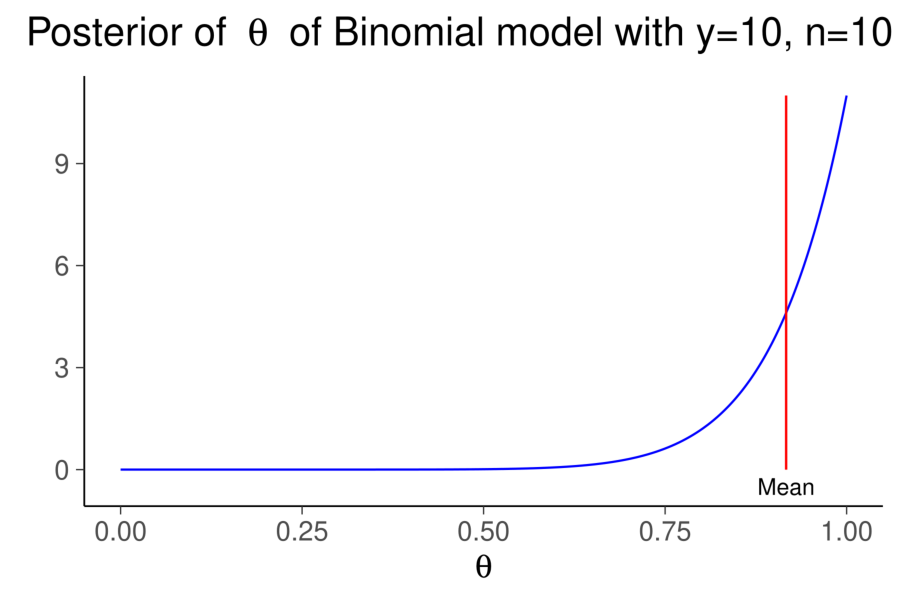
\includegraphics[width=10cm]{dbbeta10.pdf}
  \end{center}

\end{frame}

\begin{frame}{Predictive distribution}

  \begin{itemize}
  \item {\color{blue} Prior predictive} distribution for new $\tilde{y}$ (discrete)
    \begin{align*}
      p(\tilde{y}=1|M) &= \int_0^1 p(\tilde{y}=1|\theta,M){\color{blue}p(\theta|M)}d\theta
    \end{align*}
  \item {\color{red} Posterior predictive} distribution for new $\tilde{y}$ (discrete)
    \begin{align*}
      p(\tilde{y}=1|y,n,M) &= \int_0^1 p(\tilde{y}=1|\theta,y,n,M){\color{red}p(\theta|y,n,M)}d\theta
    \end{align*}
  \end{itemize}
\end{frame}

\begin{frame}{Left handedness}

  \begin{itemize}
  \item<+-> If we would like to provide scissors for all students, how
    many left handed scissors we would need?
    \begin{itemize}
    \item related to consumer behavior analysis and A/B testing
  \end{itemize}
\item<+-> Make a guess of how many left handed there are now
  \begin{itemize}
  \item<+-> tell your guess to the next one
  \end{itemize}
\end{itemize}  

\end{frame}

\begin{frame}{Left handedness}

  \vspace{-0.5\baselineskip}
  \begin{itemize}
  \item<+-> What we know and don't know
    \begin{itemize}
    \item $N=L+R$ is the total number of students in the lecture hall,
      $N$ is known in the beginning
    \item<+-> $L$ and $R$ are the number of left and right handed students, not known before we start asking
    \item<+-> $n=l+r$ is the number of students we have asked
    \item<+-> $l$ and $r$ are the numbers of left and right handed students from the students we asked
    \item<+-> we also know that $l \leq L \leq (N-r)$ and $r \leq R \leq (N-l)$
    \end{itemize}
  \item<+-> After observing $n$ students with $l$ left handed, what we
    know about $L$?
    \begin{itemize}
    \item We define $L=l+\tilde{l}$, where $\tilde{l}$ is the
      unobserved number of left handed students among those who we did
      not yet ask
    \item We know $l$, $r$, and $N$, and want to predict $\tilde{l}$ and $L$
    \end{itemize}
  \item<+-> {\color{blue} Posterior} distribution for
    $\theta$ is $\Beta(\alpha+l, \beta+r)$
  \item<+-> {\color{red} Posterior predictive} distribution for
    $\displaystyle\tilde{l}$ is\\
    $\BetaBinomial(\tilde{l} | N-n, \alpha+l, \beta+r)=\int_0^1\Bin(\tilde{l} | N-n, \theta)\Beta(\theta | \alpha+l, \beta+r)d\theta$
  \end{itemize}
  
\end{frame}

%%% handedness demo

\begin{frame}{Justification for uniform prior}

  \begin{itemize}
  \item $p({\color{red}\theta}|M)=1$ if
    \begin{itemize}
    \item[1)] we want the prior predictive distribution to be uniform
      \begin{equation*}
        p(y|n,M) = \frac{1}{n+1}, \quad y=0,\ldots,n
      \end{equation*}
      \begin{itemize}
      \item nice justification as it is based on observables $y$ and $n$
      \end{itemize}
    \item<2->[2)] we think all values of ${\color{red}\theta}$ are equally likely
      % Laplace "principle of insufficient reason"
    \end{itemize} 
  \end{itemize}

\end{frame}

\begin{frame}{Left handedness}

  \vspace{-0.5\baselineskip}
  \begin{itemize}
  \item What we know and don't know
    \begin{itemize}
    \item $N=L+R$ is the total number of students in the lecture hall,
      $N$ is known in the beginning
    \item $L$ and $R$ are the number of left and right handed students, not known before we start asking
    \item $n=l+r$ is the number of students we have asked
    \item $l$ and $r$ are the numbers of left and right handed students from the students we asked
    \item we also know that $l \leq L \leq (N-r)$ and $r \leq R \leq (N-l)$
    \end{itemize}
  \item After observing $n$ students with $l$ left handed, what we
    know about $L$?
    \begin{itemize}
    \item We define $L=l+\tilde{l}$, where $\tilde{l}$ is the
      unobserved number of left handed students among those who we did
      not yet ask
    \item We know $l$, $r$, and $N$, and want to predict $\tilde{l}$ and $L$
    \end{itemize}
  \item {\color{blue} Posterior} distribution for
    $\theta$ is $\Beta(\alpha+l, \beta+r)$
  \item {\color{red} Posterior predictive} distribution for
    $\displaystyle\tilde{l}$ is\\
    $\BetaBinomial(\tilde{l} | N-n, \alpha+l, \beta+r)=\int_0^1\Bin(\tilde{l} | N-n, \theta)\Beta(\theta | \alpha+l, \beta+r)d\theta$
  \item {\small Demo: \url{https://handedness.streamlit.app}}
  \end{itemize}
  
\end{frame}
%%% priors

\begin{frame}{Priors}

  \begin{itemize}
  \item Conjugate prior (BDA3 p. 35)
  \item Noninformative prior (BDA3 p. 51)
  \item Proper and improper prior (BDA3 p. 52)
  \item Weakly informative prior (BDA3 p. 55)
  \item Informative prior (BDA3 p. 55)
  \item Prior sensitivity (BDA3 p. 38)
  \end{itemize}

\end{frame}

\begin{frame}{Conjugate prior}

  \begin{itemize}
  \item Prior and posterior have the same form
    \begin{itemize}
    \item only for exponential family distributions (plus for
      some irregular cases)
    \end{itemize}
  \item Used to be important for computational reasons, and still
    sometimes used for special models to allow partial analytic
    marginalization (Ch 3)
    \begin{itemize}
    \item with Hamiltonian Monte Carlo / NUTS used e.g. in Stan no
      computational benefit
    \end{itemize}
  \end{itemize}
  
\end{frame}

\begin{frame}{Beta prior for Binomial model}

  \begin{itemize}
  \item Prior \vskip -1.5\baselineskip
    \begin{align*}
      \text{Beta}({\color{red} \theta}|\alpha,\beta) \propto {\color{red} \theta}^{\alpha-1}
      (1-{\color{red} \theta})^{\beta-1}
    \end{align*}
  \item Posterior
    \vskip -1.5\baselineskip
    \begin{align*}
      p({\color{red} \theta}|y,n,M) & \propto {\color{red} \theta}^y(1-{\color{red} \theta})^{n-y}
                                      {\color{red} \theta}^{\alpha-1} (1-{\color{red} \theta})^{\beta-1}\\
                                    &\uncover<2->{ \propto
                                      {\color{red} \theta}^{y+\alpha-1} (1-{\color{red} \theta})^{n-y+\beta-1}}\\
      \uncover<3->{\text{after normalization}} &\\
      \uncover<3->{p({\color{red} \theta}|y,n,M)}
                                    &\uncover<3->{ = \text{Beta}({\color{red} \theta}|\alpha+y,\beta+n-y)}
    \end{align*}
    \vskip -2mm
  \item<4-> $(\alpha-1)$ and $(\beta-1)$ can be considered to be the
    number of prior observations
  \item<4-> Uniform prior when $\alpha=1$ and $\beta=1$ 
  \end{itemize}
\end{frame}

% \begin{frame}{Placenta previa}

%   \begin{itemize}
%   \item Beta prior centered on population average 0.485
%   \end{itemize}
%   \only<1>{\includegraphics[width=11cm,trim=0 190 0 0,clip]{figs/demo2_2.pdf}}
%   \only<2>{\includegraphics[width=11cm,trim=0 135 0 0,clip]{figs/demo2_2.pdf}}
%   \only<3>{\includegraphics[width=11cm,trim=0 60 0 0,clip]{figs/demo2_2.pdf}}
%   {\includegraphics[width=11cm,trim=0 0 0 250,clip]{figs/demo2_2.pdf}}
% \end{frame}

\begin{frame}{Benefits of integration and prior}

  \vspace{-0.5\baselineskip}
  Example: $n=10, y=10$ - uniform vs Beta(2,2) prior
  \begin{center}
    \includegraphics[width=7.8cm]{dbbeta10a.pdf}\\
    \uncover<2>{\includegraphics[width=7.8cm]{dbbeta10b.pdf}}
  \end{center}

\end{frame}

\begin{frame}{Beta prior for Binomial model}

  \begin{itemize}
  \item Posterior
    \vskip -1.5\baselineskip
    \begin{align*}
      p({\color{red} \theta}|y,n,M) = \text{Beta}({\color{red} \theta}|\alpha+y,\beta+n-y)
    \end{align*}
  \item Posterior mean
    \vskip -1\baselineskip
    \begin{align*}
      \E[{\color{red} \theta}|y] = \frac{\alpha+y}{\alpha+\beta+n}
    \end{align*}
    \begin{itemize}
    \item combination prior and likelihood information
    \item when $n\rightarrow\infty$, $\text{E}[{\color{red} \theta}|y]\rightarrow y/n$
    \end{itemize}
    \pause
  \item  Posterior variance
    \vskip -1\baselineskip
    \begin{align*}
      \Var[{\color{red} \theta}|y]=\frac{\E[{\color{red} \theta}|y](1-\E[{\color{red} \theta}|y])}{\alpha+\beta+n+1}
    \end{align*}
    \begin{itemize}
    \item decreases when $n$ increases
    \item when $n\rightarrow\infty$, $\text{Var}[{\color{red} \theta}|y]\rightarrow 0$
    \end{itemize}      
  \end{itemize}

\end{frame}

% 2022: 43:30

\begin{frame}{Noninformative prior, proper and improper prior}

  \begin{itemize}
  \item Vague, flat, diffuse, or noninformative
    \begin{itemize}
    \item try to ``to let the data speak for themselves''
    \item flat is not non-informative
    \item flat can be stupid
    \item making prior flat somewhere can make it non-flat somewhere
      else
    \end{itemize}
  \item Proper prior has $\int p(\theta) = 1$
  \item Improper prior density doesn't have a finite integral
    \begin{itemize}
    \item the posterior can still sometimes be proper
    \end{itemize}
  \end{itemize}
  
\end{frame}

% \begin{frame}

%   \frametitle{Jeffrey's prior}

%   \begin{itemize}
%   \item Prior which is invariant to transformation of variables
%   \item Fisher's information matrix (more in Chapter 4) is $I(\theta)$, where
%     $\displaystyle I(\theta)_{ij}=E\left(-\frac{\partial^2 l}{\partial
%       \theta_i\partial\theta_j} \right)$ 
%   \item Jeffrey's prior is
%     \begin{align*}
        %         p(\theta) \propto \text{det}(I(\theta))^{1/2}
        %       \end{align*}
        %         \item<2-> E.g.\\
        %         $y \sim \Bin(n,\theta): \quad p(\theta)\propto \theta^{-1/2}(1-\theta)^{-1/2}$\\
        %         $y \sim N(\mu,\sigma^2): \quad p(\mu,\sigma^2)\propto 1/\sigma^2$
        %         \item<3-> May produce improper priors or too vague priors
        %         \end{itemize}

        %         \end{frame}

        %         \begin{frame}

        %         \frametitle{Noninformative Beta prior for Binomial model}

        %         \begin{itemize}
        %         \item Uniform prior is $\Beta(1,1)$
        %         \item<2-> Jeffreys prior is $\Beta(\frac{1}{2},\frac{1}{2})$
        %         \item<3-> $\Beta(0,0)$
        %         \begin{itemize}
        %         \item improper prior
        %         \item posterior is also improper if $y=0$ or $y=n$
        %         \end{itemize}
        %         \end{itemize}

        %         \end{frame}

\begin{frame}{Weakly informative priors}

  \begin{itemize}
  \item Weakly informative priors produce computationally better
    behaving posteriors
    \begin{itemize}
    \item quite often there's at least some knowledge about the
      scale
    \item useful also if there's more information from previous
      observations, but not certain how well that information is
      applicable in a new case uncertainty
    \end{itemize}
    \pause
  \item Construction
    \begin{itemize}
    \item Start with some version of a noninformative prior distribution and then add enough
      information so that inferences are constrained to be reasonable.
    \item Start with a strong, highly informative prior and broaden it to account for uncertainty
      in one's prior beliefs and in the applicability of any historically based prior distribution
      to new data.
    \end{itemize}
  \item Stan team prior choice recommendations \url{https://github.com/stan-dev/stan/wiki/Prior-Choice-Recommendations}
  \end{itemize}

\end{frame}

%%% handedness prior
\begin{frame}{Informative prior for left handedness}

  \begin{itemize}
  \item Papadatou-Pastou et al. (2020). Human handedness: A meta-analysis.
    Psychological Bulletin, 146(6), 481–524. \url{https://doi.org/10.1037/bul0000229}
    \begin{itemize}
    \item totaling 2\,396\,170 individuals
    \item varies between 9.3\% and 18.1\%, depending on how handedness is measured
    \item varies between countries and in time
    \end{itemize}
  \end{itemize}
  \only<2>{\includegraphics[width=9cm,trim=1300 550 0 240,clip]{figs/left_handed_infographic.png}\\}
  \only<3>{\includegraphics[width=9cm,trim=0 600 1400 240,clip]{figs/left_handed_infographic.png}\\}
  \only<2-3>{\tiny Fig from \url{https://www.reddit.com/r/dataisbeautiful/comments/s9x1ya/history_of_lefthandedness_oc/}}
  \only<4>{\vspace{0.5\baselineskip}\includegraphics[width=8cm]{figs/beta_8_60_prior.pdf}}
  
\end{frame}

\begin{frame}{Left handedness}

  \vspace{-0.5\baselineskip}
  \begin{itemize}
  \item What we know and don't know
    \begin{itemize}
    \item $N=L+R$ is the total number of students in the lecture hall,
      $N$ is known in the beginning
    \item $L$ and $R$ are the number of left and right handed students, not known before we start asking
    \item $n=l+r$ is the number of students we have asked
    \item $l$ and $r$ are the numbers of left and right handed students from the students we asked
    \item we also know that $l \leq L \leq (N-r)$ and $r \leq R \leq (N-l)$
    \end{itemize}
  \item After observing $n$ students with $l$ left handed, what we
    know about $L$?
    \begin{itemize}
    \item We define $L=l+\tilde{l}$, where $\tilde{l}$ is the
      unobserved number of left handed students among those who we did
      not yet ask
    \item We know $l$, $r$, and $N$, and want to predict $\tilde{l}$ and $L$
    \end{itemize}
  \item {\color{blue} Posterior} distribution for
    $\theta$ is $\Beta(\alpha+l, \beta+r)$
  \item {\color{red} Posterior predictive} distribution for
    $\displaystyle\tilde{l}$ is\\
    $\BetaBinomial(\tilde{l} | N-n, \alpha+l, \beta+r)=\int_0^1\Bin(\tilde{l} | N-n, \theta)\Beta(\theta | \alpha+l, \beta+r)d\theta$
  \item {\small Demo: \url{https://handedness.streamlit.app}}
  \end{itemize}
  
\end{frame}

\begin{frame}{Benefits of integration and prior}

  \begin{itemize}
  \item Left handed simulation with $L=30$ left handed and $N=300$ total
  \end{itemize}
  
  \only<1>{\hspace{-1cm}\includegraphics[width=11.5cm]{figs/lefthand_simulation_phat.pdf}}
  \only<2>{\hspace{-1cm}\includegraphics[width=11.5cm]{figs/lefthand_simulation_yhat.pdf}}

\end{frame}

% \begin{frame}{Benefits of integration and prior}

%   \begin{itemize}
%   \item Left handed simulation with true $\theta=0.1$ and $N=300$
%     \begin{itemize}
%     \item repeated 10\,000 times
%     \item average predictive probability for guessing $L$ after $n \leq N$ observations
%     \end{itemize}
%   \end{itemize}
  
%   \hspace{-1cm}\includegraphics[width=11.5cm]{figs/lefthand_simulation_epp_new.pdf}

% \end{frame}

\begin{frame}{Benefits of integration and prior}

  \begin{itemize}
  \item Left handed simulation with true $\theta=0.1$ and $N=300$
    \begin{itemize}
    \item repeated 10\,000 times
    \item average log predictive probability for guessing $L$ after $n \leq N$ observations
    \end{itemize}
  \end{itemize}
  
  \hspace{-1cm}\includegraphics[width=11.5cm]{figs/lefthand_simulation_logscore_new.pdf}

\end{frame}

        %         \begin{frame}{Example of informative prior}

        %         \begin{itemize}
        %         \item The percentage of girl births is remarkably stable at about
        %         48.8\% girls, rarely varying by more than 0.5\% from this rate
        %         \only<2-3>{\item There was a study on the percentage of girl births among
        %         parents in attractiveness categories 1--5 (assessed by
        %         interviewers in a face-to-face survey)}
        %         \end{itemize}
        %         \begin{center}
        %         \only<3>{\includegraphics[width=9cm]{sexratio_bayes_1.pdf}}
        %         \only<4>{\includegraphics[width=9cm]{sexratio_bayes_2.pdf}}
        %         \end{center}
        %         \end{frame}

        %         \begin{frame}{Example of weakly informative prior}

        %         \begin{itemize}
        %         \item Gabry et al (2019). Visualization in Bayesian workflow.
        %         \only<1>{
        %         \begin{itemize}
        %         \item Estimation of human exposure to air pollution from
        %         particulate matter measuring less than 2.5 microns in diameter
        %         (PM$_{2.5}$)
        %         \item A recent report estimated that PM$_{2.5}$ is responsible for three
        %         million deaths worldwide each year (Shaddick et al, 2017)
        %         \end{itemize}
        %         }
        %         \end{itemize}
        %         \begin{center}
        %         \only<2>{\includegraphics[width=10cm]{map-data.png}\\Satellite estimates and ground monitor locations}
        %         \only<3>{\includegraphics[width=6.5cm]{plot2_bigger.png}}
        %         \end{center}
        %         \end{frame}

        %         \begin{frame}{Example of weakly informative prior}

        %         \begin{center}
        %         \only<1>{\includegraphics[width=11cm]{pm25_pp1a.pdf}}
        %         \only<2>{\includegraphics[width=11cm]{pm25_pp1b.pdf}}
        %         \only<3>{\includegraphics[width=11cm]{pm25_pp2.pdf}}
        %         \end{center}
        %         \end{frame}

\begin{frame}{Effect of incorrect priors?}
  
  \begin{itemize}
  \item Introduce bias, but often still produce smaller estimation
    error because the variance is reduced
    \begin{itemize}
    \item bias-variance tradeoff
    \end{itemize}
  \end{itemize}  
  
\end{frame}

\begin{frame}{Structural information \only<1-2>{in predicting future}\only<3>{-- Prophet by Facebook}}

  \only<1>{\hspace*{-2.5cm}\includegraphics[width=16cm]{rstan_downloads_forecast.pdf}}
  \only<2>{\hspace*{-2.5cm}\includegraphics[width=16cm]{rstan_downloads_forecast_zoomed.pdf}}
  \only<3>{\hspace*{-.5cm}\includegraphics[width=11.25cm]{rstan_downloads_components.pdf}}
  
\end{frame}

        %         skip rest in video
\begin{frame}{Binomial: unknown $\theta$}

  Sometimes conditioning on the model $M$ is explicitly shown
  
  \begin{itemize}
  \item {\color{blue}Posterior} with Bayes rule (function of ${\color{red}\theta}$, continuous)
    \begin{equation*}
      p({\color{red}\theta}|y,n,M)=\frac{p(y|{\color{red}\theta},n,M)p({\color{red}\theta}|n,M)}{p(y|n,M)}
    \end{equation*}
    where $p(y|n,M)=\int p(y|\theta,n,M)p(\theta|n,M) d\theta$
    \vspace{0.5\baselineskip}
    \uncover<2->{\begin{itemize}
      \item makes it more clear that likelihood and prior are both part
        of the model
      \item makes it more clear that there is no absolute probability
        for $p(y|n)$, but it depends on the model $M$
      \item in case of two models, we can evaluate marginal likelihoods
        $p(y|n,M_1)$ and $p(y|n,M_2)$ (more in Ch 7)
      \item<3-> usually dropped to make the notation more concise
      \end{itemize}}
  \end{itemize}

\end{frame}

\begin{frame}{Sufficient statistics}

  \begin{itemize}
  \item<+-> The quantity $t(y)$ is said to be a {\em sufficient statistic}
    for $\theta$, because the likelihood for $\theta$ depends on the
    data $y$ only through the value of $t(y)$.
  \item<+-> For binomial model the sufficient statistics are $y$ and
    $n$ (the order doesn't matter)
  \end{itemize}

\end{frame}

%%% demos

\begin{frame}{Posterior visualization and inference demos}

  \begin{itemize}
  \item demo2\_3: Simulate samples from Beta(438,544), and draw
    a histogram of $\theta$ with quantiles.
  \end{itemize}
  \vspace{-\baselineskip}
  \begin{center}
    \includegraphics[width=11cm]{figs/demo2_3.pdf}
  \end{center}
\end{frame}

\begin{frame}{Posterior visualization and inference demos}

  \begin{itemize}
  \item demo2\_4: Compute posterior distribution in a grid.
  \end{itemize}
  \includegraphics[width=11cm]{figs/demo2_4a.pdf}
\end{frame}

\begin{frame}{Posterior visualization and inference demos}

  \begin{itemize}
  \item demo2\_4: Sample using the inverse-cdf method.
  \end{itemize}
  \includegraphics[width=11cm]{figs/demo2_4b.pdf}
\end{frame}

\begin{frame}{Algae}
  \framesubtitle{Assignment}

  Algae status is monitored in 274 sites at Finnish lakes and rivers. 
  The observations for the 2008 algae status at each site are presented
  in file \emph{algae.(rda|txt)} ('0': no algae, '1': algae present). 
        %         In year 2008 blue-green algae was observed at 44 sites. 
  Let $\theta$ be the probability of a monitoring site having detectable
  blue-green algae levels. 

  \begin{itemize}
  \item Use a binomial model for observations and a $\Beta(2,10)$ prior.
  \item What can you say about the value of the unknown $\theta$?
  \item Experiment how the result changes if you change the prior.
  \end{itemize}

\end{frame}

\begin{frame}{Binomial model with $\theta=f(x)$}

  \begin{itemize}
  \item Next week you learn how the binomial model parameter $\theta$
    can depend on some other measurement $x$
  \end{itemize}
  
  \includegraphics[width=10.5cm]{figs/helicopter_stable_brms.pdf}
  
\end{frame}

%%% normal

\begin{frame}{Normal / Gaussian}

  \begin{itemize}
  \item Observations ${\color{red}y}$ real valued
  \item Mean $\theta$ and variance $\sigma^2$ (or deviation $\sigma$)\\
    This week assume $\sigma^2$ known (preparing for the next week)
  \end{itemize}
  \vskip -2mm
  \begin{align*}
    p({\color{red}y}|\theta)&=\frac{1}{\sqrt{2\pi}\sigma}\exp\left(-\frac{1}{2\sigma^2}({\color{red}y}-\theta)^2\right)\\
    {\color{red}y} & \sim \N(\theta,\sigma^2)
  \end{align*}

  \begin{center}
    \includegraphics[clip]{kuva2b_1}
  \end{center}
\end{frame}

\begin{frame}{Reasons to use Normal distribution}

  \begin{itemize}
  \item Normal distribution often justified based on central limit theorem
  \item More often used due to the computational convenience or tradition
  \end{itemize}

\end{frame}

%% skip in video

\begin{frame}{Central limit theorem*}

  \begin{itemize}
  \item De Moivre, Laplace, Gauss, Chebysev, Liapounov, Markov, et al.
  \item Given certain conditions, distribution of sum (and mean) of
    random variables approach Gaussian distribution as
    $n \rightarrow \infty$
  \item Problems
    \begin{itemize}
    \item does not hold for distributions with infinite variance,
      e.g., Cauchy
    \item<2-> may require large $n$,\\ e.g.
      Binomial, when $\theta$ close to $0$ or $1$
    \item<3-> does not hold if one the variables has much larger scale
    \end{itemize}
  \end{itemize}

\end{frame}

        %         \begin{frame}
        %         \frametitle{Normal distribution - conjugate prior for $\theta$}

        %         \begin{itemize}
        %         \item Assume $\sigma^2$ known
        %         \begin{align*}
        %                             &\text{Likelihood} & p(y|\theta) & \propto
                                                                         %                                                                          \exp\left(-\frac{1}{2\sigma^2}(y-\theta)^2\right)\\ \\
        %                             &\text{Prior} & p(\theta) & \propto \exp\left(-\frac{1}{2\tau_0^2}(\theta-\mu_0)^2\right)
                                                                  %       \end{align*}
                                                                  %                                                                   \end{itemize}
                                                                  %                                                                   \end{frame}

\begin{frame}{Normal distribution - conjugate prior for $\theta$}

  \begin{itemize}
  \item Assume $\sigma^2$ known
    \begin{align*}
      &\text{Likelihood} & p(y|{\color{red}\theta}) & \propto
                                                      \exp\left(-\frac{1}{2\sigma^2}(y-{\color{red}\theta})^2\right)\\ \\
      &\text{Prior} & p({\color{red}\theta}) & \propto
                                               \exp\left(-\frac{1}{2\tau_0^2}({\color{red}\theta}-\mu_0)^2\right)\\ \\
      & & \uncover<2->{\exp(a)\exp(b)} & \uncover<2->{= \exp(a+b)} \\ \\
      &\uncover<3->{ \text{Posterior}}&
                                        \uncover<3->{p({\color{red}\theta}|y)& \propto \exp\left(-\frac{1}{2}\left[ \frac{(y-{\color{red}\theta})^2}{\sigma^2}+\frac{({\color{red}\theta}-\mu_0)^2}{\tau_0^2} \right]\right)}
    \end{align*}
  \end{itemize}

\end{frame}

                                                                               %                                                                                \note{  exp(a)*exp(b)=exp(a+b)}

\begin{frame}{Normal distribution - conjugate prior for $\theta$}

  \begin{itemize}
  \item Posterior (highly recommended to do BDA 3 Ex 2.14a)
    \vskip -5mm
    \begin{align*}
      & &
          p({\color{red}\theta}|y)&\propto \exp\left(-\frac{1}{2}\left[
                                    \frac{(y-{\color{red}\theta})^2}{\sigma^2}+\frac{({\color{red}\theta}-\mu_0)^2}{\tau_0^2} \right]\right) \\ 
      & & & \propto \exp \left(-\frac{1}{2\tau_1^2}({\color{red}\theta}-\mu_1)^2
            \right)
    \end{align*}
    \begin{equation*}
      {\color{red}\theta}|y \sim \N(\mu_1,\tau_1^2), \quad
      \text{where} \quad
      \mu_1=\frac{\frac{1}{\tau_0^2}\mu_0+\frac{1}{\sigma^2}y}{\frac{1}{\tau_0^2}+\frac{1}{\sigma^2}} \quad  \text{and}  \quad \frac{1}{\tau_1^2} = \frac{1}{\tau_0^2}+\frac{1}{\sigma^2}
    \end{equation*}
    \vskip -2mm
    \pause
  \item 1/variance = precision
  \item Posterior precision = prior precision + data precision
  \item Posterior mean is precision weighted mean
  \end{itemize}


\end{frame}

\begin{frame}{Normal distribution - example}

  \only<1>{\includegraphics[width=11cm]{pguess.pdf}}
  \only<2>{\includegraphics[width=11cm]{pguessprior.pdf}}
  \only<3>{\includegraphics[width=11cm]{ppost.pdf}}
  
\end{frame}

\begin{frame}{Normal distribution - conjugate prior for $\theta$}

  \begin{itemize}
  \item Several observations -- use chain rule
  \end{itemize}

\end{frame}

\begin{frame}{Normal distribution - conjugate prior for $\theta$}

  \begin{itemize}
  \item Several observations $y=(y_1,\ldots,y_n)$
    \begin{align*}
      p({\color{red}\theta}|y) = \N({\color{red}\theta}|\mu_n,\tau_n^2)
    \end{align*}
    \vskip -6mm
    \begin{align*}
      \text{where} \quad
      \mu_n=\frac{\frac{1}{\tau_0^2}\mu_0+\frac{n}{\sigma^2}\bar{y}}{\frac{1}{\tau_0^2}+\frac{n}{\sigma^2}} \quad
      \text{ja} \quad \frac{1}{\tau_n^2} = \frac{1}{\tau_0^2}+\frac{n}{\sigma^2}
    \end{align*}
  \item If $\tau_0^2=\sigma^2$, prior corresponds to one virtual observation with value $\mu_0$
    \pause
  \item If $\tau_0\rightarrow\infty$ when $n$ fixed\\
    or if $n\rightarrow\infty$ when $\tau_0$ fixed
    \begin{equation*}
      p({\color{red}\theta}|y) \approx \N({\color{red}\theta}|\bar{y},\sigma^2/n)
    \end{equation*}
  \end{itemize}

\end{frame}

\begin{frame}{Normal distribution - conjugate prior for $\theta$}

  \begin{itemize}
  \item Posterior predictive distribution
    \begin{align*}
      p({\color{red}\tilde{y}}|y)&=\int p({\color{red}\tilde{y}}|\theta)p(\theta|y) d\theta \\
      p({\color{red}\tilde{y}}|y)& \propto\int
                                   \exp\left(-\frac{1}{2\sigma^2}({\color{red}\tilde{y}}-\theta)^2\right)\exp\left(-\frac{1}{2\tau_1^2}(\theta-\mu_1)^2\right) d\theta \\
      ~&~\\ 
      {\color{red}\tilde{y}}|y &\sim \N(\mu_1,\sigma^2+\tau_1^2)
    \end{align*}
  \item Predictive variance = observation model variance $\sigma^2$ + \\
    posterior variance $\tau_1^2$

  \end{itemize}

\end{frame}

\begin{frame}{Normal model}

  \begin{itemize}
  \item Gets more interesting when both mean and variance are unknown
    \begin{itemize}
    \item next week
    \end{itemize}
  \item<2-> The mean can be also a function of covariates
    \begin{itemize}
    \item e.g. normal linear regression $y \sim \N(\alpha + \beta x, \sigma^2)$
    \end{itemize}
  \item<3-> Gaussian processes, Kalman filters, variational
    inference, Laplace approximaion, etc.
  \end{itemize}
\end{frame}

\begin{frame}{Some other one parameter models}

  \begin{itemize}
  \item Poisson, useful for count data (e.g. in epidemiology)
  \item Exponential, useful for time to an event (e.g. particle decay)
  \end{itemize}
  
\end{frame}

\begin{frame}{Poisson model for count data}

  \begin{itemize}
  \item Number of traffic deaths per year (by Liikenneturva)
  \end{itemize}

  \vspace{\baselineskip}
  
  \only<+>{\includegraphics[height=7cm]{figs/traffic1.pdf}}
  \only<+>{\includegraphics[height=7cm]{figs/traffic2.pdf}}
  \only<+>{\includegraphics[height=7cm]{figs/traffic3.pdf}}
  \only<+>{\includegraphics[height=7cm]{figs/traffic4.pdf}}
  \only<+>{\includegraphics[height=7cm]{figs/traffic5.pdf}}
  
\end{frame}

\begin{frame}{Thinking priors}

  \begin{itemize}
  \item Make a guess of some quantities and then find out useful
    prior information for that. E.g.
    \begin{itemize}
    \item proportion of students using MS Windows vs. Apple macOS vs. Linux
    \item proportion of students who are longer than 1.9m
    \item proportion of students, who submitted the first assignment,
      attending the next lecture
    \item proportion of students, who submitted the first assignment,
      submitting the last assignment
    \end{itemize}
  \end{itemize}
  
\end{frame}

\end{document}

%%% Local Variables: 
%%% TeX-PDF-mode: t
%%% TeX-master: t
%%% End: 
